
%% bare_jrnl.tex
%% V1.4b
%% 2015/08/26
%% by Michael Shell
%% see http://www.michaelshell.org/
%% for current contact information.
%%
%% This is a skeleton file demonstrating the use of IEEEtran.cls
%% (requires IEEEtran.cls version 1.8b or later) with an IEEE
%% journal paper.
%%
%% Support sites:
%% http://www.michaelshell.org/tex/ieeetran/
%% http://www.ctan.org/pkg/ieeetran
%% and
%% http://www.ieee.org/

%%*************************************************************************
%% Legal Notice:
%% This code is offered as-is without any warranty either expressed or
%% implied; without even the implied warranty of MERCHANTABILITY or
%% FITNESS FOR A PARTICULAR PURPOSE! 
%% User assumes all risk.
%% In no event shall the IEEE or any contributor to this code be liable for
%% any damages or losses, including, but not limited to, incidental,
%% consequential, or any other damages, resulting from the use or misuse
%% of any information contained here.
%%
%% All comments are the opinions of their respective authors and are not
%% necessarily endorsed by the IEEE.
%%
%% This work is distributed under the LaTeX Project Public License (LPPL)
%% ( http://www.latex-project.org/ ) version 1.3, and may be freely used,
%% distributed and modified. A copy of the LPPL, version 1.3, is included
%% in the base LaTeX documentation of all distributions of LaTeX released
%% 2003/12/01 or later.
%% Retain all contribution notices and credits.
%% ** Modified files should be clearly indicated as such, including  **
%% ** renaming them and changing author support contact information. **
%%*************************************************************************


% *** Authors should verify (and, if needed, correct) their LaTeX system  ***
% *** with the testflow diagnostic prior to trusting their LaTeX platform ***
% *** with production work. The IEEE's font choices and paper sizes can   ***
% *** trigger bugs that do not appear when using other class files.       ***                          ***
% The testflow support page is at:
% http://www.michaelshell.org/tex/testflow/



\documentclass[journal]{IEEEtran}
%
% If IEEEtran.cls has not been installed into the LaTeX system files,
% manually specify the path to it like:
% \documentclass[journal]{../sty/IEEEtran}





% Some very useful LaTeX packages include:
% (uncomment the ones you want to load)


% *** MISC UTILITY PACKAGES ***
%
%\usepackage{ifpdf}
% Heiko Oberdiek's ifpdf.sty is very useful if you need conditional
% compilation based on whether the output is pdf or dvi.
% usage:
% \ifpdf
%   % pdf code
% \else
%   % dvi code
% \fi
% The latest version of ifpdf.sty can be obtained from:
% http://www.ctan.org/pkg/ifpdf
% Also, note that IEEEtran.cls V1.7 and later provides a builtin
% \ifCLASSINFOpdf conditional that works the same way.
% When switching from latex to pdflatex and vice-versa, the compiler may
% have to be run twice to clear warning/error messages.






% *** CITATION PACKAGES ***
%
%\usepackage{cite}
% cite.sty was written by Donald Arseneau
% V1.6 and later of IEEEtran pre-defines the format of the cite.sty package
% \cite{} output to follow that of the IEEE. Loading the cite package will
% result in citation numbers being automatically sorted and properly
% "compressed/ranged". e.g., [1], [9], [2], [7], [5], [6] without using
% cite.sty will become [1], [2], [5]--[7], [9] using cite.sty. cite.sty's
% \cite will automatically add leading space, if needed. Use cite.sty's
% noadjust option (cite.sty V3.8 and later) if you want to turn this off
% such as if a citation ever needs to be enclosed in parenthesis.
% cite.sty is already installed on most LaTeX systems. Be sure and use
% version 5.0 (2009-03-20) and later if using hyperref.sty.
% The latest version can be obtained at:
% http://www.ctan.org/pkg/cite
% The documentation is contained in the cite.sty file itself.






% *** GRAPHICS RELATED PACKAGES ***
%
\ifCLASSINFOpdf
  % \usepackage[pdftex]{graphicx}
  % declare the path(s) where your graphic files are
  % \graphicspath{{../pdf/}{../jpeg/}}
  % and their extensions so you won't have to specify these with
  % every instance of \includegraphics
  % \DeclareGraphicsExtensions{.pdf,.jpeg,.png}
\else
  % or other class option (dvipsone, dvipdf, if not using dvips). graphicx
  % will default to the driver specified in the system graphics.cfg if no
  % driver is specified.
  % \usepackage[dvips]{graphicx}
  % declare the path(s) where your graphic files are
  % \graphicspath{{../eps/}}
  % and their extensions so you won't have to specify these with
  % every instance of \includegraphics
  % \DeclareGraphicsExtensions{.eps}
\fi
% graphicx was written by David Carlisle and Sebastian Rahtz. It is
% required if you want graphics, photos, etc. graphicx.sty is already
% installed on most LaTeX systems. The latest version and documentation
% can be obtained at: 
% http://www.ctan.org/pkg/graphicx
% Another good source of documentation is "Using Imported Graphics in
% LaTeX2e" by Keith Reckdahl which can be found at:
% http://www.ctan.org/pkg/epslatex
%
% latex, and pdflatex in dvi mode, support graphics in encapsulated
% postscript (.eps) format. pdflatex in pdf mode supports graphics
% in .pdf, .jpeg, .png and .mps (metapost) formats. Users should ensure
% that all non-photo figures use a vector format (.eps, .pdf, .mps) and
% not a bitmapped formats (.jpeg, .png). The IEEE frowns on bitmapped formats
% which can result in "jaggedy"/blurry rendering of lines and letters as
% well as large increases in file sizes.
%
% You can find documentation about the pdfTeX application at:
% http://www.tug.org/applications/pdftex


\usepackage{booktabs} % For formal tables
\usepackage{graphicx}
\usepackage{amsmath,amssymb,amsfonts}
\usepackage{algorithmic}
\usepackage{subfigure}


% *** MATH PACKAGES ***
%
%\usepackage{amsmath}
% A popular package from the American Mathematical Society that provides
% many useful and powerful commands for dealing with mathematics.
%
% Note that the amsmath package sets \interdisplaylinepenalty to 10000
% thus preventing page breaks from occurring within multiline equations. Use:
%\interdisplaylinepenalty=2500
% after loading amsmath to restore such page breaks as IEEEtran.cls normally
% does. amsmath.sty is already installed on most LaTeX systems. The latest
% version and documentation can be obtained at:
% http://www.ctan.org/pkg/amsmath





% *** SPECIALIZED LIST PACKAGES ***
%
%\usepackage{algorithmic}
% algorithmic.sty was written by Peter Williams and Rogerio Brito.
% This package provides an algorithmic environment fo describing algorithms.
% You can use the algorithmic environment in-text or within a figure
% environment to provide for a floating algorithm. Do NOT use the algorithm
% floating environment provided by algorithm.sty (by the same authors) or
% algorithm2e.sty (by Christophe Fiorio) as the IEEE does not use dedicated
% algorithm float types and packages that provide these will not provide
% correct IEEE style captions. The latest version and documentation of
% algorithmic.sty can be obtained at:
% http://www.ctan.org/pkg/algorithms
% Also of interest may be the (relatively newer and more customizable)
% algorithmicx.sty package by Szasz Janos:
% http://www.ctan.org/pkg/algorithmicx




% *** ALIGNMENT PACKAGES ***
%
%\usepackage{array}
% Frank Mittelbach's and David Carlisle's array.sty patches and improves
% the standard LaTeX2e array and tabular environments to provide better
% appearance and additional user controls. As the default LaTeX2e table
% generation code is lacking to the point of almost being broken with
% respect to the quality of the end results, all users are strongly
% advised to use an enhanced (at the very least that provided by array.sty)
% set of table tools. array.sty is already installed on most systems. The
% latest version and documentation can be obtained at:
% http://www.ctan.org/pkg/array


% IEEEtran contains the IEEEeqnarray family of commands that can be used to
% generate multiline equations as well as matrices, tables, etc., of high
% quality.




% *** SUBFIGURE PACKAGES ***
%\ifCLASSOPTIONcompsoc
%  \usepackage[caption=false,font=normalsize,labelfont=sf,textfont=sf]{subfig}
%\else
%  \usepackage[caption=false,font=footnotesize]{subfig}
%\fi
% subfig.sty, written by Steven Douglas Cochran, is the modern replacement
% for subfigure.sty, the latter of which is no longer maintained and is
% incompatible with some LaTeX packages including fixltx2e. However,
% subfig.sty requires and automatically loads Axel Sommerfeldt's caption.sty
% which will override IEEEtran.cls' handling of captions and this will result
% in non-IEEE style figure/table captions. To prevent this problem, be sure
% and invoke subfig.sty's "caption=false" package option (available since
% subfig.sty version 1.3, 2005/06/28) as this is will preserve IEEEtran.cls
% handling of captions.
% Note that the Computer Society format requires a larger sans serif font
% than the serif footnote size font used in traditional IEEE formatting
% and thus the need to invoke different subfig.sty package options depending
% on whether compsoc mode has been enabled.
%
% The latest version and documentation of subfig.sty can be obtained at:
% http://www.ctan.org/pkg/subfig




% *** FLOAT PACKAGES ***
%
%\usepackage{fixltx2e}
% fixltx2e, the successor to the earlier fix2col.sty, was written by
% Frank Mittelbach and David Carlisle. This package corrects a few problems
% in the LaTeX2e kernel, the most notable of which is that in current
% LaTeX2e releases, the ordering of single and double column floats is not
% guaranteed to be preserved. Thus, an unpatched LaTeX2e can allow a
% single column figure to be placed prior to an earlier double column
% figure.
% Be aware that LaTeX2e kernels dated 2015 and later have fixltx2e.sty's
% corrections already built into the system in which case a warning will
% be issued if an attempt is made to load fixltx2e.sty as it is no longer
% needed.
% The latest version and documentation can be found at:
% http://www.ctan.org/pkg/fixltx2e


%\usepackage{stfloats}
% stfloats.sty was written by Sigitas Tolusis. This package gives LaTeX2e
% the ability to do double column floats at the bottom of the page as well
% as the top. (e.g., "\begin{figure*}[!b]" is not normally possible in
% LaTeX2e). It also provides a command:
%\fnbelowfloat
% to enable the placement of footnotes below bottom floats (the standard
% LaTeX2e kernel puts them above bottom floats). This is an invasive package
% which rewrites many portions of the LaTeX2e float routines. It may not work
% with other packages that modify the LaTeX2e float routines. The latest
% version and documentation can be obtained at:
% http://www.ctan.org/pkg/stfloats
% Do not use the stfloats baselinefloat ability as the IEEE does not allow
% \baselineskip to stretch. Authors submitting work to the IEEE should note
% that the IEEE rarely uses double column equations and that authors should try
% to avoid such use. Do not be tempted to use the cuted.sty or midfloat.sty
% packages (also by Sigitas Tolusis) as the IEEE does not format its papers in
% such ways.
% Do not attempt to use stfloats with fixltx2e as they are incompatible.
% Instead, use Morten Hogholm'a dblfloatfix which combines the features
% of both fixltx2e and stfloats:
%
% \usepackage{dblfloatfix}
% The latest version can be found at:
% http://www.ctan.org/pkg/dblfloatfix




%\ifCLASSOPTIONcaptionsoff
%  \usepackage[nomarkers]{endfloat}
% \let\MYoriglatexcaption\caption
% \renewcommand{\caption}[2][\relax]{\MYoriglatexcaption[#2]{#2}}
%\fi
% endfloat.sty was written by James Darrell McCauley, Jeff Goldberg and 
% Axel Sommerfeldt. This package may be useful when used in conjunction with 
% IEEEtran.cls'  captionsoff option. Some IEEE journals/societies require that
% submissions have lists of figures/tables at the end of the paper and that
% figures/tables without any captions are placed on a page by themselves at
% the end of the document. If needed, the draftcls IEEEtran class option or
% \CLASSINPUTbaselinestretch interface can be used to increase the line
% spacing as well. Be sure and use the nomarkers option of endfloat to
% prevent endfloat from "marking" where the figures would have been placed
% in the text. The two hack lines of code above are a slight modification of
% that suggested by in the endfloat docs (section 8.4.1) to ensure that
% the full captions always appear in the list of figures/tables - even if
% the user used the short optional argument of \caption[]{}.
% IEEE papers do not typically make use of \caption[]'s optional argument,
% so this should not be an issue. A similar trick can be used to disable
% captions of packages such as subfig.sty that lack options to turn off
% the subcaptions:
% For subfig.sty:
% \let\MYorigsubfloat\subfloat
% \renewcommand{\subfloat}[2][\relax]{\MYorigsubfloat[]{#2}}
% However, the above trick will not work if both optional arguments of
% the \subfloat command are used. Furthermore, there needs to be a
% description of each subfigure *somewhere* and endfloat does not add
% subfigure captions to its list of figures. Thus, the best approach is to
% avoid the use of subfigure captions (many IEEE journals avoid them anyway)
% and instead reference/explain all the subfigures within the main caption.
% The latest version of endfloat.sty and its documentation can obtained at:
% http://www.ctan.org/pkg/endfloat
%
% The IEEEtran \ifCLASSOPTIONcaptionsoff conditional can also be used
% later in the document, say, to conditionally put the References on a 
% page by themselves.




% *** PDF, URL AND HYPERLINK PACKAGES ***
%
%\usepackage{url}
% url.sty was written by Donald Arseneau. It provides better support for
% handling and breaking URLs. url.sty is already installed on most LaTeX
% systems. The latest version and documentation can be obtained at:
% http://www.ctan.org/pkg/url
% Basically, \url{my_url_here}.




% *** Do not adjust lengths that control margins, column widths, etc. ***
% *** Do not use packages that alter fonts (such as pslatex).         ***
% There should be no need to do such things with IEEEtran.cls V1.6 and later.
% (Unless specifically asked to do so by the journal or conference you plan
% to submit to, of course. )


% correct bad hyphenation here
\hyphenation{op-tical net-works semi-conduc-tor}


\begin{document}
%
% paper title
% Titles are generally capitalized except for words such as a, an, and, as,
% at, but, by, for, in, nor, of, on, or, the, to and up, which are usually
% not capitalized unless they are the first or last word of the title.
% Linebreaks \\ can be used within to get better formatting as desired.
% Do not put math or special symbols in the title.
\title{Revisiting Binary trees for\\ Efficient FPGA-based NoC Implementations}
%
%
% author names and IEEE memberships
% note positions of commas and nonbreaking spaces ( ~ ) LaTeX will not break
% a structure at a ~ so this keeps an author's name from being broken across
% two lines.
% use \thanks{} to gain access to the first footnote area
% a separate \thanks must be used for each paragraph as LaTeX2e's \thanks
% was not built to handle multiple paragraphs
%

\author{Kizheppatt~Vipin,~\IEEEmembership{Member,~IEEE}% <-this % stops a space
\thanks{K. Vipin is with the Department of Electrical and Computer Engineering, Nazarbayev University, Astana,
Kazakhstan, 010000 e-mail: vipin.kizheppatt@nu.edu.kz}}% <-this % stops a space


% note the % following the last \IEEEmembership and also \thanks - 
% these prevent an unwanted space from occurring between the last author name
% and the end of the author line. i.e., if you had this:
% 
% \author{....lastname \thanks{...} \thanks{...} }
%                     ^------------^------------^----Do not want these spaces!
%
% a space would be appended to the last name and could cause every name on that
% line to be shifted left slightly. This is one of those "LaTeX things". For
% instance, "\textbf{A} \textbf{B}" will typeset as "A B" not "AB". To get
% "AB" then you have to do: "\textbf{A}\textbf{B}"
% \thanks is no different in this regard, so shield the last } of each \thanks
% that ends a line with a % and do not let a space in before the next \thanks.
% Spaces after \IEEEmembership other than the last one are OK (and needed) as
% you are supposed to have spaces between the names. For what it is worth,
% this is a minor point as most people would not even notice if the said evil
% space somehow managed to creep in.



% The paper headers
\markboth{IEEE TRANSACTIONS ON VERY LARGE SCALE INTEGRATION (VLSI) SYSTEMS, VOL. 25, NO. 2, FEBRUARY 2017}%
{K. Vipin \MakeLowercase{\textit{et al.}}: Revisiting Binary trees for Efficient FPGA-based NoC Implementations}
% The only time the second header will appear is for the odd numbered pages
% after the title page when using the twoside option.
% 
% *** Note that you probably will NOT want to include the author's ***
% *** name in the headers of peer review papers.                   ***
% You can use \ifCLASSOPTIONpeerreview for conditional compilation here if
% you desire.




% If you want to put a publisher's ID mark on the page you can do it like
% this:
%\IEEEpubid{0000--0000/00\$00.00~\copyright~2015 IEEE}
% Remember, if you use this you must call \IEEEpubidadjcol in the second
% column for its text to clear the IEEEpubid mark.



% use for special paper notices
%\IEEEspecialpapernotice{(Invited Paper)}




% make the title area
\maketitle


\begin{abstract}
Binary tree topology generally fails to attract network on chip (NoC) implementations due to its low bisection bandwidth.
Fat trees are proposed to alleviate this issue by using increasingly thicker links to connect switches towards the root node.
This scheme is very efficient in interconnected networks such as computer networks, which use generic switches for interconnection.
In an NoC context, especially for field programmable gate arrays (FPGAs), fat trees require more complex switches as we move higher in the hierarchy.
This restricts the maximum clock frequency at which the network operates and offsets the higher bandwidth achieved through using fatter links.
In this paper we discuss the implementation of a binary tree-based NoC, which achieves better bandwidth by varying the clock frequency between the switches as we move higher in the hierarchy.
This scheme enables using simpler switch architecture thus supporting higher maximum frequency of operation.
The effect on bandwidth and resource requirement of this architecture is compared with other FPGA-based NoCs for different network sizes and traffic patterns.
\end{abstract}

\begin{IEEEkeywords}
network on chip, topology, binary tree, FPGA
\end{IEEEkeywords}

%\IEEEpeerreviewmaketitle
\section{Introduction}
Network on Chip (NoC) architectures enable high performance, scalable and power efficient multi-core systems for modern compute and communication intensive applications.
Researchers have proposed different NoC topologies such as mesh, ring, torus, binary trees, star etc., each having varying degrees of quality of service, bandwidth and latency~\cite{Dally2003}.
Despite their simple architecture and routing algorithms, binary trees are generally not attractive for NoC implementations.
It is mainly because of its lower bisection bandwidth.
Fat trees are proposed as a remedy to improve the bandwidth by adding more number of links when moving towards the root node.
This solution works well in traditional interconnect networks such as computer networks~\cite{Shainer2011}.
In a NoC environment, their advantage is limited since more complex switches have to be used in higher hierarchy.
This limits the maximum supported clock frequency of the network thus bringing down the system performance. 

Theoretically instead of increasing the link width between tree levels, increasing the clock frequency between them should provide the same benefit.
In traditional computer networks this may not be possible since the network interfaces operate on predefined standards which restricts the frequency of operation.
In an NoC environment, this is very much possible since all the compute instances are with in the same chip and are not restricted by any physical protocol. 
Modern FPGAs support asynchronous FIFOs, which makes the implementation of such asynchronous switches easier.
These switches have simpler architecture than fat tree switches and support better clock frequency.
But they are more resource intensive compared to traditional binary trees.

Although asynchronous NoCs are proposed before for integrated circuits, a quantitative analysis is missing in the literature especially for FPGA implementations~\cite{Bjerregaard2005, USP2011}.
In this work we present a quantitative analysis of different tree topologies namely the binary tree, binary fat tree and asynchronous binary tree when targeting FPGA based NoC implementation. 
The main contributions of this work are
\begin{itemize}
\item detailed design of an open-source globally asynchronous-locally synchronous (GALS) binary tree based NoC implementation targeting Xilinx FPGAs
\item performance evaluation of the proposed infrastructure with traditional binary trees and the state-of-the-art open source binary fat tree, torus and mesh topologies
\item analysis of trade-off points for the different implementations when targeting FPGAs
\end{itemize}
The remainder of this paper is organized as, Section~\ref{sec:background} discusses the relevant background, Section~\ref{sec:arch} discusses the architecture of the proposed NoC, Section~\ref{sec:result} discussed the performance metrics and ~\ref{sec:conclusion} concludes the paper and gives the future research directions.
\section{Background}
\label{sec:background}
Network on chip is an interconnect approach that helps different IPs and subsystems in a chip to communicate with each other in an efficient and scalable manner. 
In this approach each processing element (PE) is connected to a switch and multiple switches are interconnected to form a network.
A PE could be a processor core, a DSP core or an IP block.
The network infrastructure helps in routing data from one PE to another in the form of data packets. 
NoCs have found varying applications such as image and signal processing~\cite{Joshi2007}, multi-processor systems~\cite{Bertozzi2005}, virtual machine implementations~\cite{Mathias2006} etc.
Based on how the switches are interconnected, there are different NoC topologies such as mesh, torus, tree, ring, star, BFT etc. as shown in Fig.~\ref{fig:topologies}~\cite{ORTINOBON201624}.

\begin{figure}[t]
\centering
   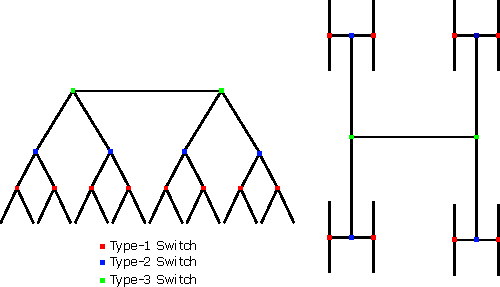
\includegraphics[width=\columnwidth]{Figures/HNoC.pdf}
   \caption{(a)A binary tree topology utilizing switches operating at different clock frequencies (b) The tree as an H-tree for better floorplanning on the FPGA}
   \label{fig:btree}
\end{figure}

In a mesh topology every switch, except the ones on the edges, is connected to 4 other neighboring switches.
A torus topology is similar to mesh but cyclic in nature.
In a binary tree, switches are arranged in a hierarchy.
Each switch has a parent node and two child nodes.
Unlike mesh and torus where each switch has a corresponding PE, in a tree topology only the switches at the bottom most level~(leaf nodes) are connected to PEs.

\begin{figure}[t]
\centering
   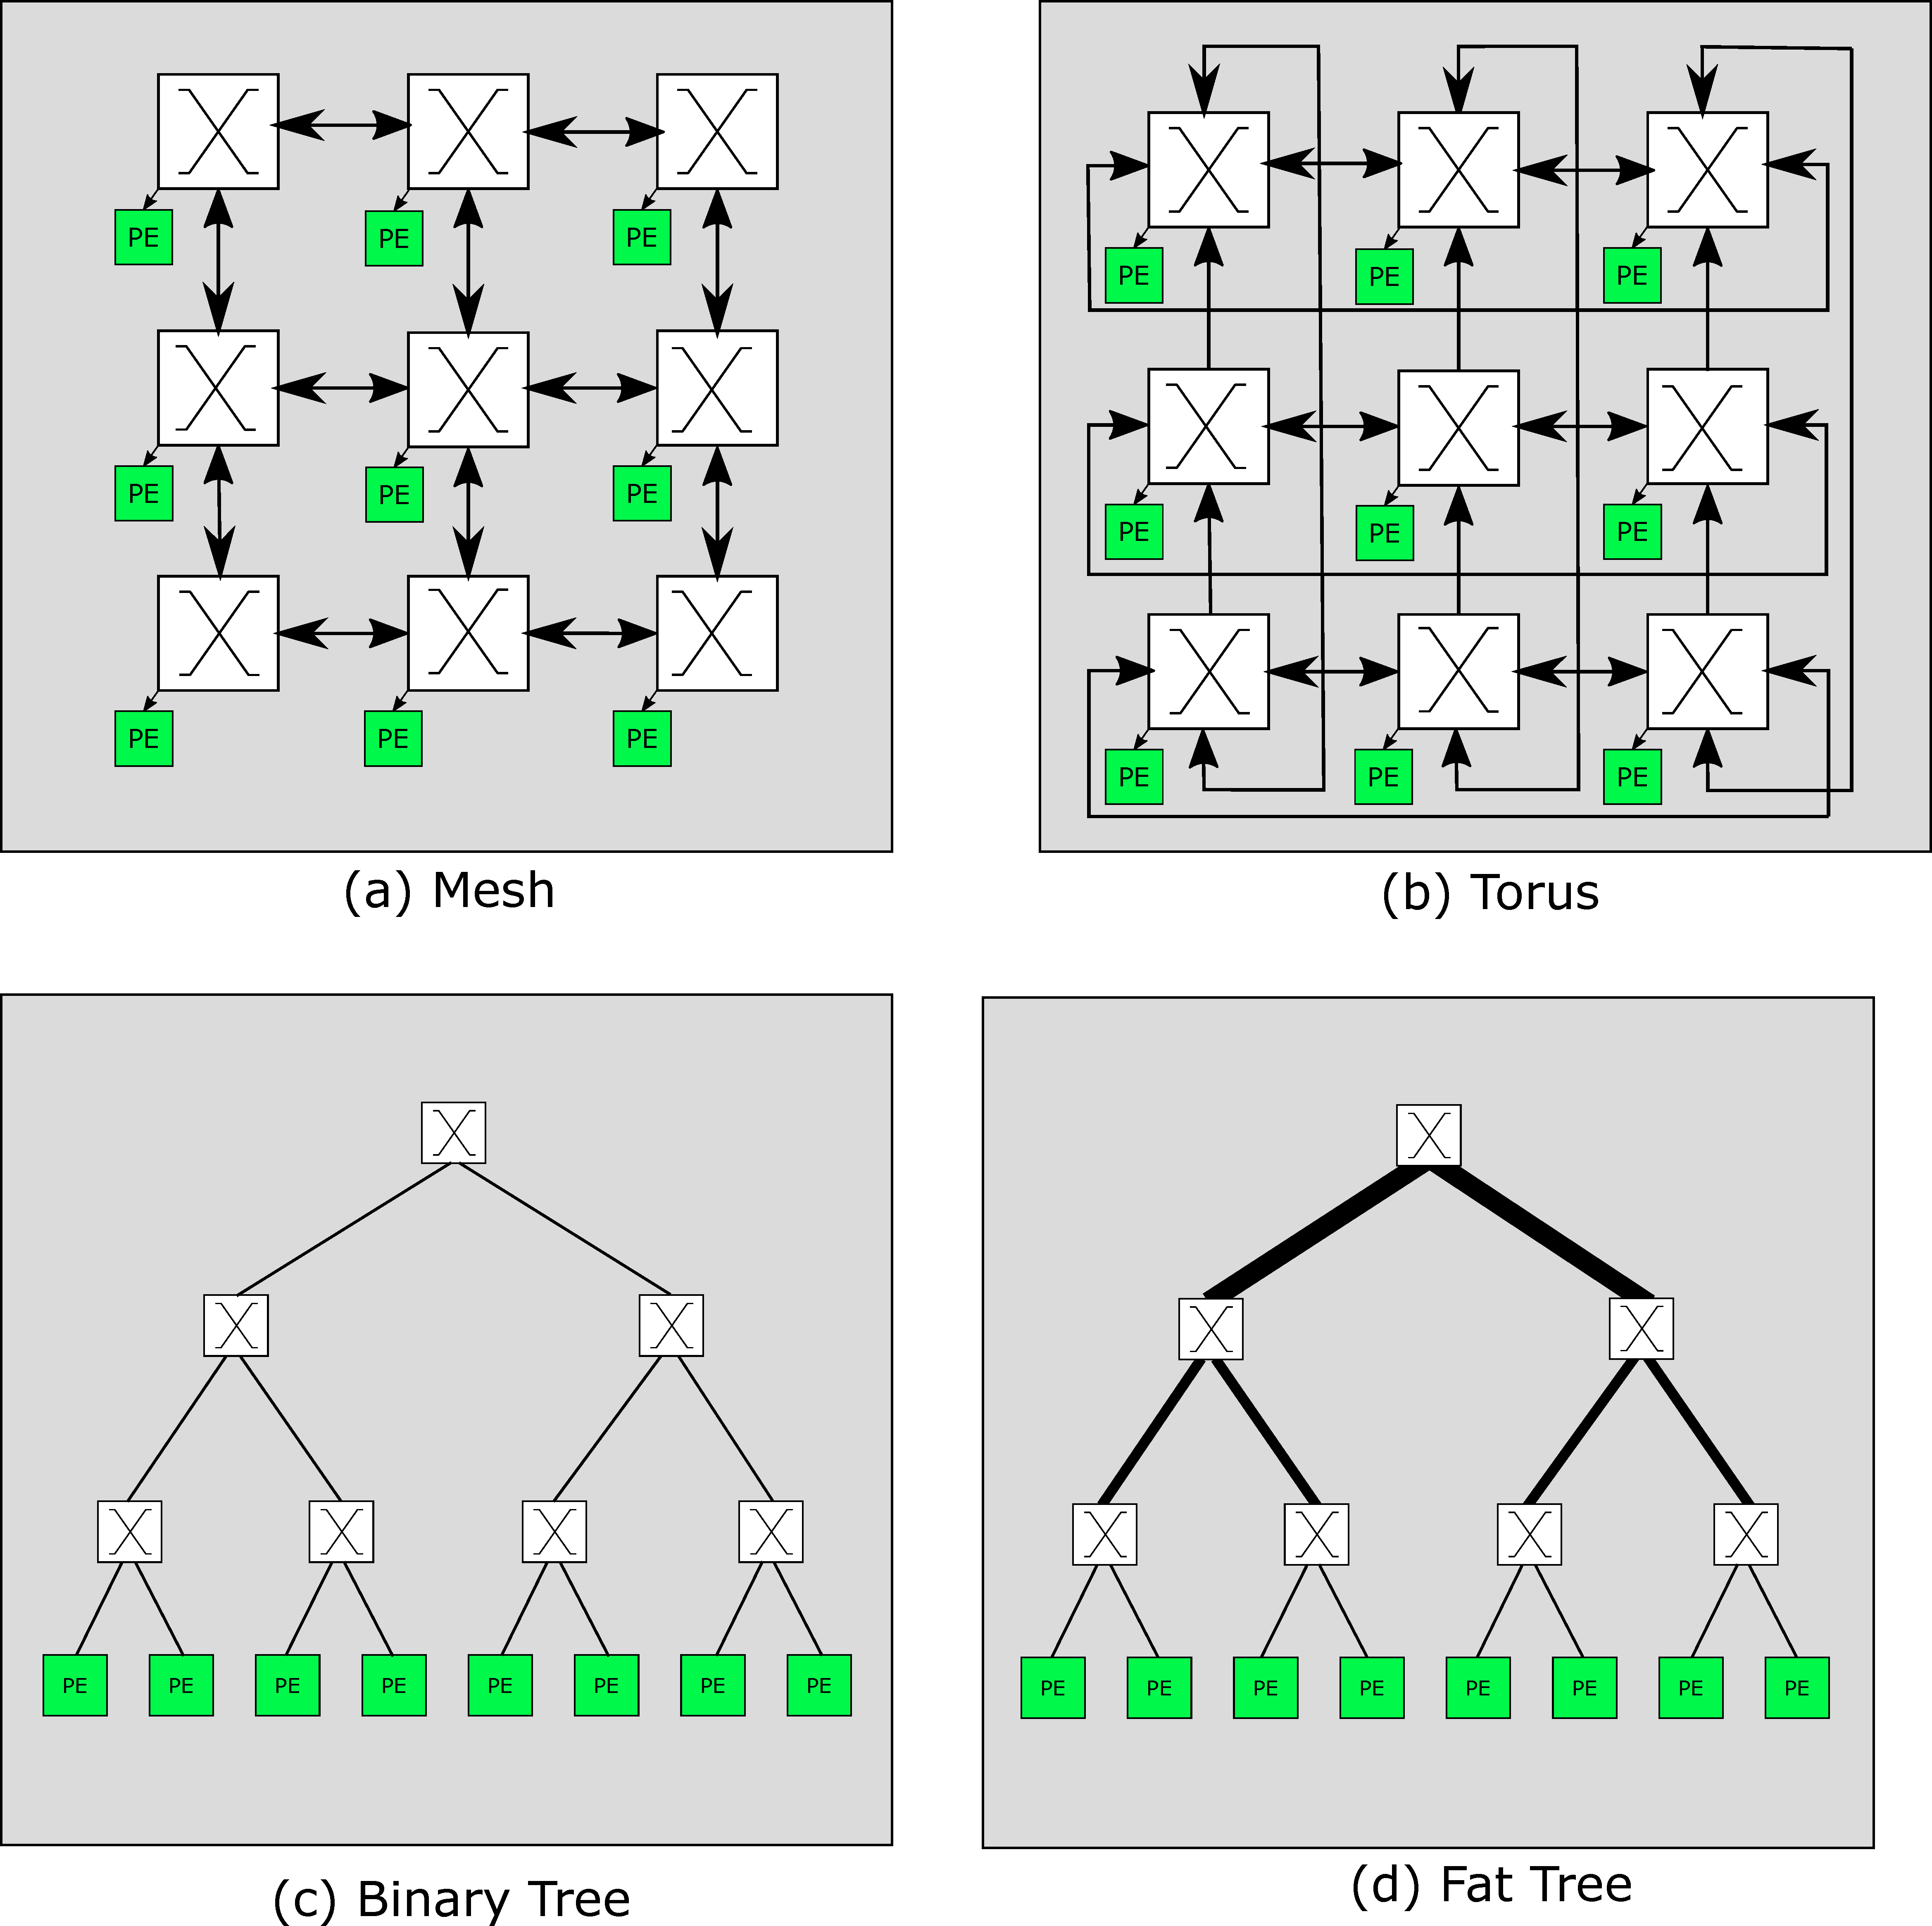
\includegraphics[width=\columnwidth]{Figures/topologies.pdf}
   \caption{Different NoC topologies}
   \label{fig:topologies}
\end{figure}

For interconnected networks, an important performance parameter is the bisection bandwidth~\cite{Wen-Chung2012}.
It is defined as the minimum bandwidth between two equal partitions of the network.
For a mesh topology, it is $\sqrt{n}*B$, where \emph{n} is the number of switches and \emph{B} is the bandwidth of a single link.
For torus, it is twice that of mesh but for a binary tree, it is only \emph{B}.
To address this issue, instead of using a single link between switches, more links can be used between them as we go higher in the tree hierarchy.
Such topology is called a fat tree~\cite{Leiserson1985,Ohring1995}. 
Although this will improve the bisection bandwidth, the switches in the upper hierarchy becomes more and more complex.
In this work we analyze whether using asynchronous switches with same link width can provide similar performance of fat trees while keeping relatively simpler switches.

\begin{figure}[t]
\centering
   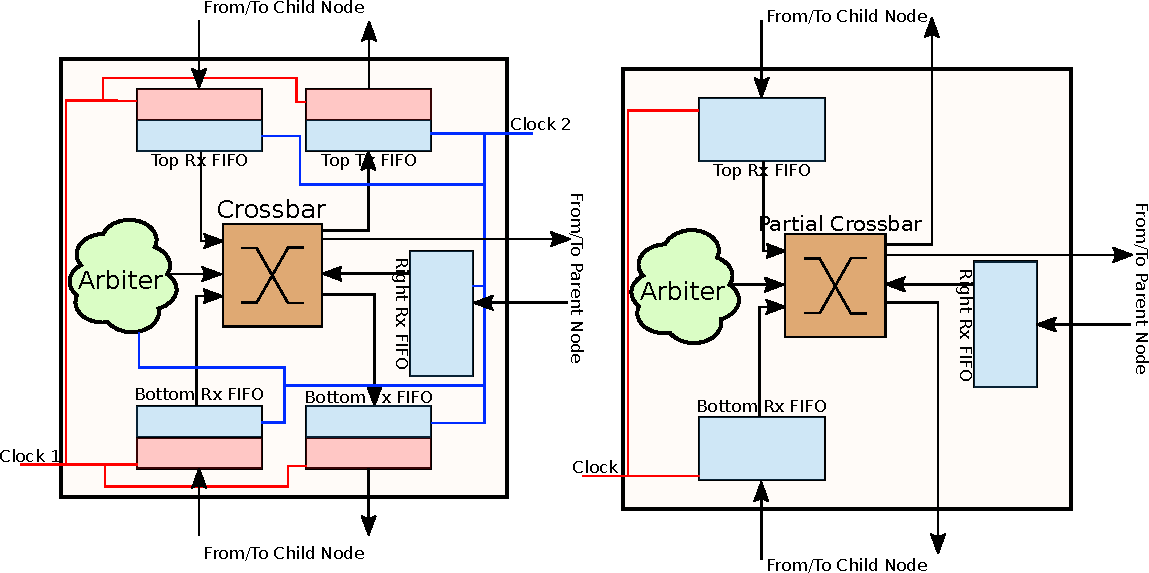
\includegraphics[width=\columnwidth]{Figures/switch1_2.pdf}
   \caption{Architecture of the different switches used in the AsyncBTree. (a) Type-1 switch used with the leaf nodes (PEs), with complete cross bar switch and asynchronous 
   FIFOs with receive and transmit interfaces (b) Type-2 switch used in intermediate nodes with partial crossbar switch and synchronous FIFOs (c) Type-3 switches used in intermediate
   switches with partial cross bar and asynchronous FIFOs with receive and transmit interfaces.}
   \label{fig:switchArch}
\end{figure}

There have been previous efforts to develop NoC architectures specifically targeting FPGAs.
CONNECT NoC generator is the most popular among them~\cite{papa_connect_fpga2012}.
CONNECT is inspired by the fact that FPGAs have a large routing infrastructure available compared to memory and logic elements and tries to exploit it. 
It supports different NoC topologies and uses a single stage pipeline mechanism  to minimize hardware and latency. 
It has low operating frequency and is still quite resource intensive as seen in Section~\ref{sec:result}. 
Split-merge is another NoC infrastructure developed at University of Pennsylvania~\cite{Huan2012}.
It tries to overcome the limited clock performance of CONNECT at the expense of few more resources.


To the best of our knowledge, there have been no previous efforts to implement asynchronous switch-based NoCs targeting FPGAs. 
In this work we give a quantitative analysis of the performance of asynchronous binary trees.
We compare their performance with traditional and fat trees as well as other popular FPGA NoCs.
The binary tree implementations are available as open-source for other researchers to verify and to improvise the designs.
\section{Architecture}
\label{sec:arch}

An AsyncBTree tries to achieve better performance compared to a conventional binary tree and binary fat tree in terms of resource utilization and throughput by applying FPGA and topology specific optimizations and using asynchronous links between different tree levels.
Fig.~\ref{fig:btree} shows the architecture of an AsyncBTree utilizing different kind of optimized switches at different levels.
The detailed architecture of the switches are discussed in Section~\ref{sec:switch}.
The binary tree is placed and routed in the FPGA as an H-tree for efficient resource utilization and better floor-planning.
Such placement also supports partial reconfiguration of a portion of the NoC in an efficient manner.
As the first optimization, the root node of the tree is removed and the switches at level-1 are directly connected.
Since the connectivity of the root node is only 2, in practical systems they act as a transparent switch.
They could be useful where packets are injected to the NoC through the root node by making its connectivity into 3.
For FPGAs external interfaces such as PCI express and Ethernet are used for injecting packets.
The hard-macros corresponding to these interfaces are situated along the periphery of the chips.
Thus it will provide better clock performance when the packets are injected from one the leaf nodes which incorporates one of these hard macros.
Removing the root node helps in reducing the resource utilization.

\begin{figure}[t]
\centering
   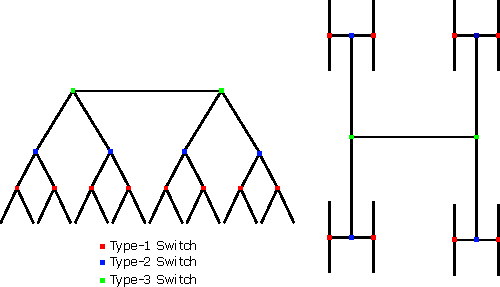
\includegraphics[width=\columnwidth]{Figures/HNoC.pdf}
   \caption{(a)A binary tree topology utilizing switches operating at different clock frequencies (b) The tree as an H-tree for better floorplanning on the FPGA}
   \label{fig:btree}
\end{figure}

\begin{figure}[t]
\centering
   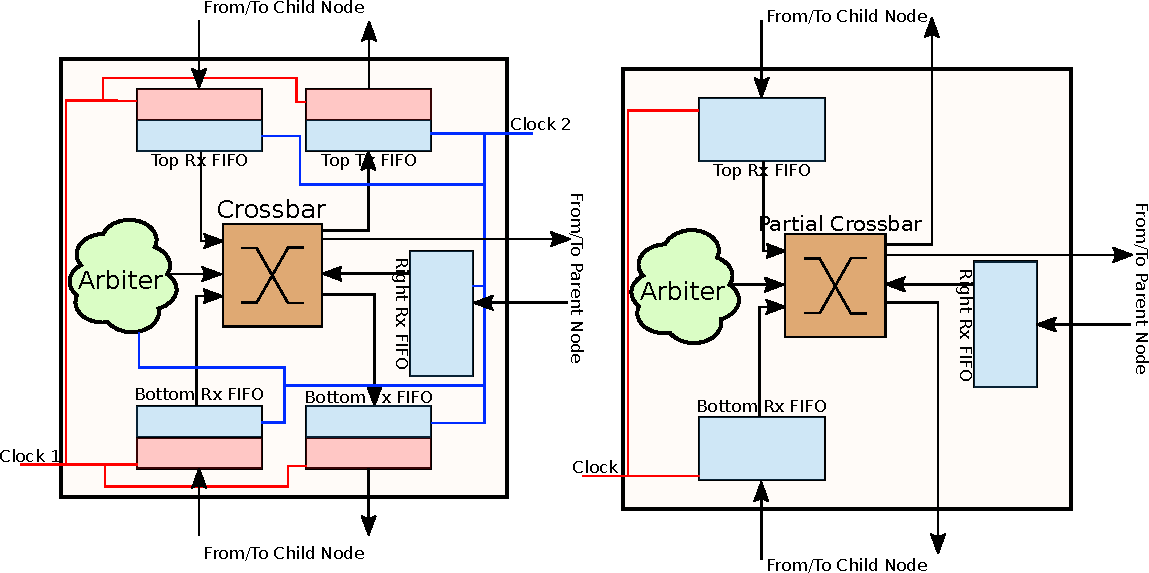
\includegraphics[width=\columnwidth]{Figures/switch1_2.pdf}
   \caption{Architecture of the different switches used in the AsyncBTree. (a) Type-1 switch used with the leaf nodes (PEs), with complete cross bar switch and asynchrnous 
   FIFOs with receive and transmit interfaces (b) Type-2 switch used in intermediate nodes with partial crossbar switch and synchronous FIFOs (c) Type-3 switches used in intermediate
   switches with partial cross bar and asynchrnous FIFOs with receive and transmit interfaces.}
   \label{fig:switchArch}
\end{figure}

\subsection{Switches}
\label{sec:switch}
AsyncBTrees use three different kinds of switches for packet routing.
The architecture of the proposed type-1 switch is as shown in Fig.~\ref{fig:switchArch}(a).
Type-1 switches are used only in the leaf nodes for directly interfacing with PEs.
The switch has separate interface for receiving and transmitting packets from two PEs and a single interface to the parent node.
Each receive and transmit interface to/from the PEs are connected to asynchronous FIFOs.
The interface to the parent node implements a single synchronous FIFO for the receive interface but no transmit FIFO.
Thus each switch contains 5 FIFOs.

Asynchronous FIFOs can operate their read and write interfaces using independent clocks.
Depth of the FIFOs are kept very low (16) to reduce the resource utilization.
The asynchronous FIFOs receive data from the downstream ports on Clock 1 signal.
The received packets are routed to the appropriate output ports by an arbitrator through a cross-bar switch.
The read side of the receive FIFO, the write side of the transmit FIFO, the arbitrator and the cross bar works on Clock 2 signal, whose frequency will be much higher than that of Clock 1.
In order to match the performance of a binary fat tree, Clock 2 frequency should be twice as that of Clock 1.

Type-1 switches implement a full cross bar, which enables loop back of packets at the switch level.
The arbitrator internally uses flit-level round-robin arbitration scheme to select the input port when more than one port requests for the same output port.
If a single input port is requesting for a particular output port, it is given the port access until all the flits are sent out.

Fig.~\ref{fig:switchArch}(b) shows the architecture of a type-2 switch.
Type-2 switches are synchronous in nature and are similar to the switches of traditional binary trees.
These switches implement only partial cross-bar switch where an in coming packet cannot be routed back to the same port.
Since these switches are used only in intermediate levels, there is no necessity to to support loop-back since they are already implemented by Type-1 switches.
This simplifies the switch design and helps in reducing resource utilization.

Type-3 switches (Fig.~\ref{fig:switchArch}(b)) are similar to type-1 switches except that they implement only a partial cross-bar similar to type-2 switches.
Type-2 and type-3 switches can be interchangeably used in the proposed architecture. 
Theoretically to match the performance of a binary fat tree, AsyncBTrees should be implementing type-3 switches at every level with increasing clock frequencies.
But in practical scenarios, doubling clock frequency at each level is not possible in FPGAs as the tree size increases.
The maximum frequency supported by modern devices are in the order of hundredes of megahertz.
Hence for practical implementations, AsyncBTrees increases the clock frequency only for alternative levels. 
Although asynchronous FIFOs can operate using same clock signal for read and write interfaces, the resource utilization of an asynchronous FIFOs is much more than its synchronous counter part for a given FIFO size.
It is because of the presence of additional circuitry for managing clock domain crossing between the read and write interfaces.
For reducing resource consumption, levels which operates on synchronous clock uses type-3 switches and levels which operate on asynchronous clock uses type-2 switches.

\subsection{Routing}
\label{sec:routing}
AyncBTree uses fixed routing based on the destination address of the packet header~\ref{fig:packet}.
The routing is flit level routing meaning each packet is expected to have the destination PE address in the packet header.
Larger packets are sent as multiple flits.
One major advantage of binary trees is the multiple packets sent from one PE to another will be always delivered in the sent order.
In other packet switched networks such as mesh or torus, the packets could be delivered in out of order depending on the routing algorithms.
In this case additional logic is required for packet reassembly and packet numbers also have to be inserted into the payload.

The routing table of each switch in AsyncBTree contains four entries corresponding to the smallest and largest PE addresses in its left sub-tree and right sub-tree.
If the destination address is with in the range of left sub-tree, it is routed left and if it is with in the range of right sub-tree the packet is sent right.
If the address is not within these ranges, the packet is routed towards the parent node.
Due to the deterministic routing policy and since the routing is at flit-level, the NoC is free of dead or livelocks.

\begin{figure}[t]
\centering
   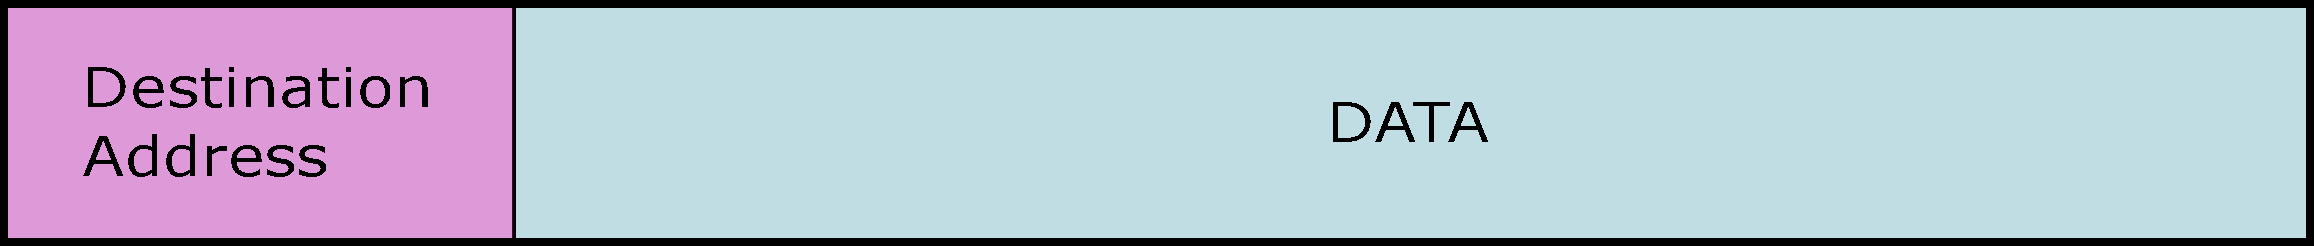
\includegraphics[width=\columnwidth]{Figures/pckt_structure.pdf}
   \caption{Packet structure}
   \label{fig:packet}
\end{figure}

\section{Flow control}
The current AsyncBTree implementation does not include virtual channels and flow control is achieved through at electrical signaling level.
The interface between switches as well as switches and PEs confirm to AXI4-stream interface.
Such interface also enables seamless integration of several vendor supported IP cores directly with the NoC.
As per AXI4-stream protocol, a successful data transfer happens only when the \emph{valid} signal from the transmitter and \emph{ready} signal from the receiver are asserted as shown in Fig.~\ref{axi}.
\section{Results and Discussion}
\label{sec:result}

In this section we discuss the implementation and performance comparison of the different NoC implementations.
All designs are modeled using Verilog HDL and extensively simulated for their functional correctness.
We use the CONNECT open-source NoC platform as the fat tree, mesh and torus references~\cite{papa_connect_fpga2012}.
The designs are simulated as well as implemented with Vivado 2017.3 targeting Xilinx xc7vx690t FPGA (VC709 evaluation board).

\input Tables/SystemResource
Table~\ref{table:systemResourceConsumption} compares the resource utilization and the maximum frequency of operation for the binary tree, AsyncBTree, and fat tree for different network sizes (number of PEs).
For all implementations, the interface between PEs and the switches are kept 32-bits wide.
As expected, binary trees are least resource intensive due to their simple switch architecture.
AsyncBTree consumes 45\% to 65\% more LUTs (look-up-tables) and about 165\% more flip flops compared to the binary tree implementation.
The multiple frequencies in the AsyncBTree rows represent the maximum clock frequency supported at different tree levels.
At the lowest level (switches connected to PEs), the clock performance is better than that of binary trees but deteriorates as going higher in the hierarchy.
This could be because of the additional pipelining present inside the asynchronous FIFOs.
This also means if AsyncBTree is used as a synchronous NoC (all tree levels are clocked by a single clock source), its resource consumption and performance will be worse than a binary tree. 

Compared to AsyncBTree, fat trees consume $\sim$3.7$\times$ LUTs but less than half the number of flip flops.
AsyncBTree requires more flip flops due to the presence of asynchronous FIFOs.
For fat trees, the impact due to complex switches can be clearly seen in the clock performance, where they are not even able to achieve 200 MHz for a high-end FPGA.
Due to the low clock performance of the NoC, the PEs also have to be under-clocked in most scenarios for overall synchronous operations.
%Otherwise synchronization FIFOs have to be inserted between PEs and the NoC switches, which will further increase the resource utilization.
Considering the fact that the number of LUTs available in 7-series Xilinx FPGAs are half of that of number of flip-flops, AsyncBTree is much lite compared fat trees at the same time given more than 4$\times$ clock performance.

\input Tables/ResourceDiffConf
Table~\ref{table:NocResourceUtilisation} lists the resource utilization and clock performance of the most popular FPGA NoC topologies namely mesh and torus.
Data shows that these topologies are quite resource intensive compared to all binary tree configurations, especially the number of LUTs.
In terms of clock performance, for larger NoC configurations, they perform better than fat trees but inferior to traditional binary trees and the proposed AsyncBTrees.

Fig.~\ref{fig:tput} and~\ref{fig:latency} compares the throughput and latency of the three implementations with different NoC sizes for different traffic patterns such as random, tornado and reverse~\cite{Bahn2008}.
The different patterns are generated based on how the destination addresses as generated for each data packet.
In each case, the PE to switch interface is clocked at the lowest frequency supported among the three implementations.
For AsyncBTree upper levels are clocked at double the frequency of lower levels, but limited by maximum supported frequency given in Table~\ref{table:systemResourceConsumption}.
It could be seen that for NoC size up to 8 PEs, AsyncBTree performance is better than or comparable to that of fat trees.
For larger tree sizes, fat trees perform better since the clock frequencies cannot be scaled beyond a limit.
If PEs run at lower clock frequencies ($\sim$50 MHz), AsyncBTree can provide better performance for NoC with up to 16 PEs. 

Fig.~\ref{fig:tputmax} and~\ref{fig:latmax} compares the throughput and latency when each implementation is running at its maximum supported frequency.
Again for smaller NoC sizes binary tree and AsyncBTree out performs fat tree for random traffic pattern.
But for larger NoC sizes fat trees are clearly advantageous.
Fig.~\ref{fig:tputmax}(a) also shows the performance of mesh topology, which is the most popular NoC topology, compared to different tree topologies.
Again for smaller NoC sizes (8 or less) AsyncTree performance is better.
Several FPGA-based multi-processor systems have 8 core or less thus AsyncBTree could be much suitable for their implementation.

Fig.~\ref{fig:tputPerf} compares the performance of each NoC compared to their resource utilization.
The total number of resources is calculated by adding the number of LUTs with the scaled number of flip-flops.
The number of flip-flops is multiplied by a factor of 0.5 since in Xilinx 7-series FPGAs there are twice the number of flip-flops compared to LUTs in every logic slice.
Synchronous binary trees clearly have an upper hand in this regard.
AsyncBTree give moderately high throughput by consuming relatively less resources.
But for larger NoC size, mesh topology is still the suitable candidate.


\begin{figure}[t]
\centering
   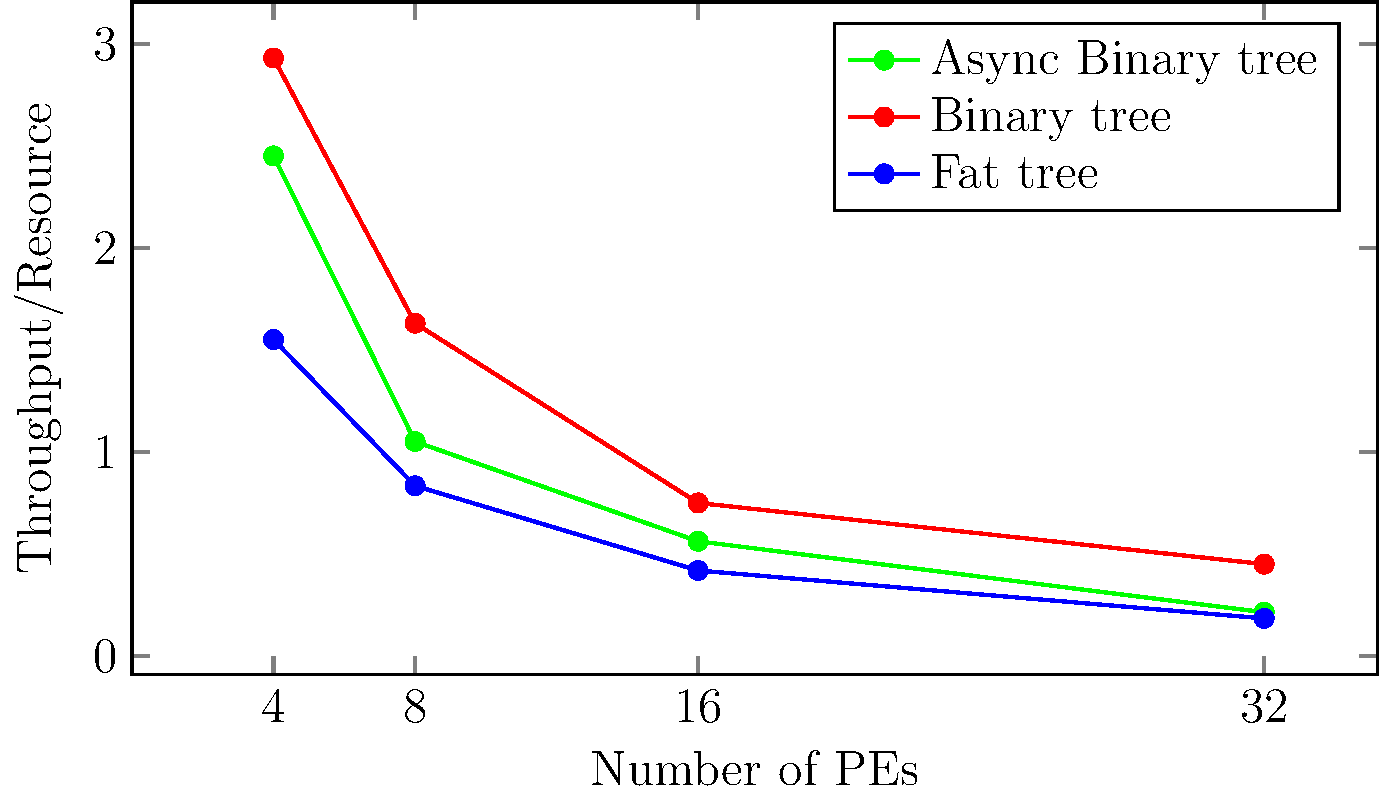
\includegraphics[width=\columnwidth]{Data/tputVsCost.pdf}
   \vspace{-5mm}
   \caption{Throughput vs cost}
   \vspace{-5mm}
      \label{fig:tputPerf}
\end{figure}

\section{Conclusion}
\label{sec:conclusion}
In this paper we discussed the implementation of an asynchronous binary tree based NoC architecture targeting FPGA implementation.
Analysis shows that FPGA archtiecture specific optimization can provide high clock performance and low resource consumption for such implementation compared to traditional fat-tree based implementations.
It also shows the advantage of fixed size interface to PEs compared to variable size interface when targeting the NoC for partial reconfiguration.
Implementation of the proposed architecture is provided as an open source enabling other researchers to verify its functionality and to use in practical NoC-based applications~\cite{hnoc}.
In the future we will be anayzing the effect of GALS-based implementation of other network topologies when targeting FPGA implementations.



\bibliographystyle{IEEEtran}
\bibliography{nocs} 

\begin{IEEEbiography}{Kizheppatt~Vipin}
Biography text here.
\end{IEEEbiography}

\end{document}
